\documentclass[12pt]{report}

%%%%%%%%%%%%%%%%%%%%%%%%%%
%%%%%% UNIT PREAMBLE %%%%% 
%%%%%%%%%%%%%%%%%%%%%%%%%%

% Basics 
\usepackage[utf8]{inputenc}
\usepackage[T1]{fontenc}
\usepackage{textcomp}
\usepackage[a4paper, left=1in, right=1in, top=1in, bottom=1in]{geometry}
\renewcommand\familydefault{\sfdefault}

\usepackage[Sonny]{fncychap}

\usepackage{amsmath,amsfonts,amsthm,amssymb,mathtools}
\usepackage[varbb]{newpxmath}
\usepackage{xfrac}
\usepackage[usenames,dvipsnames]{xcolor} % usenames, dvipsnames adds more colours
\usepackage{hhline}
\usepackage{comment}
\usepackage{tasks}
\usepackage{enumerate} 
\usepackage{enumitem} 
\usepackage{titlesec}
\usepackage[most]{tcolorbox}
\usepackage{lipsum}
\usepackage{tabularx}
\usepackage[labelfont=bf]{caption}
\usepackage{subfig}
\usepackage{pgfplots}
\usepackage{cancel} 
\usepackage{physics} 
\usepackage[bookmarks]{hyperref}
\usepackage{array}
\usepackage{float}
\usepackage{standalone}
\usepackage{graphicx}
\usepackage{forest}

% Tables 
\numberwithin{table}{section}

% Inkscape Figures
\usepackage{import}
\usepackage{xifthen}
\usepackage{pdfpages}
\usepackage{transparent}
\newcommand{\incfig}[2][1]{
    \def\svgwidth{#1\columnwidth}
    \import{../figures/}{#2.pdf_tex}
}

\pdfsuppresswarningpagegroup=1

% Chemistry
\usepackage{lewis} 
\usepackage{bohr}
\usepackage[version=4]{mhchem}

% Page setup
\hypersetup{hidelinks}
\pagenumbering{arabic}
\pagestyle{plain}
\setlength{\parindent}{0pt}

% Show subsubsections
\setcounter{tocdepth}{3}
\setcounter{secnumdepth}{3}

% Required for the Grid
\usetikzlibrary{calc}

% Section Font-Size
\titleformat{\subsubsection}
  {\normalfont\fontsize{12}{12}\bfseries}{\thesubsubsection}{1em}{}

\titleformat{\subsection}
  {\normalfont\fontsize{14}{14}\bfseries}{\thesubsection}{1em}{}

\titleformat{\section}
  {\normalfont\fontsize{16}{16}\bfseries}{\thesection}{1em}{}

% New page for each section 
\newcommand{\sectionbreak}{\clearpage}

% Section Spacing
\titlespacing{\section}{0em}{2.5em}{1em}
\titlespacing{\subsection}{0em}{2.5em}{1em}
\titlespacing{\subsubsection}{0em}{2.5em}{1em}

% TABLE COLUMN SEPARATION (USES ARRAY PACKAGE)
% \renewcommand{\arraystretch}{1.8} % changes vertical space for each cell 
% \setlength{\tabcolsep}{18pt} % changes horizontal space for each cell
% \setlength{\arrayrulewidth}{0.25mm}

% TCOLORBOX 
% \newtcolorbox[auto counter, number within=section]{definition}{colback=white,title=Example~\thetcbcounter,breakable,colframe=white,boxrule=0pt, enhanced, title style={left color=gray!60,right color=white,middle color=white},arc=0mm, titlerule=0pt, fonttitle=\bfseries\sffamily}

% Theorems 
\usepackage{thmtools}
\usepackage[framemethod=TikZ]{mdframed}

\declaretheoremstyle[
    headfont=\bfseries\sffamily\color{ProcessBlue!70!black}, bodyfont=\normalfont,
    headpunct= :,
    mdframed={
        linewidth=2pt,
        rightline=false, topline=false, bottomline=false,
        linecolor=ProcessBlue, backgroundcolor=ProcessBlue!5,
        innerbottommargin=10pt
    } ]{note}

\declaretheoremstyle[
    headfont=\bfseries\sffamily\color{NavyBlue!70!black}, 
    bodyfont=\normalfont,
    % headpunct=,
    mdframed={
        linewidth=2pt,
        rightline=false, topline=false, bottomline=false, linecolor=NavyBlue, innerbottommargin=10pt
    }
]{solution}

\declaretheoremstyle[
    headfont=\bfseries\sffamily\color{Gray!70!black}, bodyfont=\normalfont,
    % headpunct= ,
    postheadspace=\newline,
    mdframed={
        linewidth=2pt,
        rightline=false, topline=false, bottomline=false,
        linecolor=Gray, backgroundcolor=Gray!5,
        innerbottommargin=10pt
    } ]{remark}

\declaretheoremstyle[
    headfont=\bfseries\sffamily\color{Fuchsia!70!black}, bodyfont=\normalfont,
    % headpunct= ,
    mdframed={
        linewidth=2pt,
        rightline=false, topline=false, bottomline=false,
        linecolor=Fuchsia, backgroundcolor=Fuchsia!5,
        innerbottommargin=10pt
    }
]{example}

\declaretheoremstyle[
    headfont=\bfseries\sffamily\color{Fuchsia!70!black}, 
    bodyfont=\normalfont,
    % headpunct= ,
    mdframed={
        linewidth=2pt,
        rightline=false, topline=false, bottomline=false,
        linecolor=Fuchsia,
    }
]{examplesolution}

\declaretheoremstyle[
    headfont=\bfseries\sffamily\color{black!70!black}, 
    bodyfont=\normalfont,
    mdframed={
        linewidth=1pt,
        rightline=false, topline=false, bottomline=false,
        linecolor=black,
    }
]{definition}

\declaretheorem[style=solution, name=Solution, numbered=no]{solution}

\declaretheorem[style=solution, name=Derivation, numbered=no]{derivation}

\declaretheorem[style=definition, name=Definition, numberwithin=chapter]{definition}

\declaretheorem[style=note, name=Note, numbered=no]{noteswap}
\newenvironment{note}[1]{\vspace{0.5em}\begin{noteswap}[#1]}{\end{noteswap}\vspace{0.5em}}

\declaretheorem[style=remark, name=Remark, numbered=no]{remarkswap}
\newenvironment{remark}{\vspace{0.5em}\begin{remarkswap}}{\end{remarkswap}\vspace{0.5em}}

\declaretheorem[style=example, name=Example, numbered=no]{exampleswap}
% \newenvironment{example}{\vspace{0.5em}\begin{exampleswap}}{\end{exampleswap}}

\declaretheorem[style=examplesolution, name=Solution, numbered=no]{examplesolutionswap}
\newenvironment{examplesolution}{\vspace{-2em}\begin{examplesolutionswap}}{\end{examplesolutionswap}}

% Enumerate environments 
\newenvironment{2qu}
{
\begin{enumerate}[label=(\alph*)]
}
{\end{enumerate}}

\newenvironment{3qu}
{
\begin{enumerate}[label=(\roman*)]
}
{\end{enumerate}}

% Normal Environments 
\newenvironment{list0.5}
{
\begin{enumerate}
\setlength\itemsep{0.5em}
}
{\end{enumerate}}

% \titleformat{\section}{\vbox{\rule{\linewidth}{0.8pt}}\bigskip\LARGE\bfseries}{\thesection}{1em}{}

\titleformat{\section}
  {\normalfont\Large\bfseries}{\thesection}{1em}{}[{\titlerule[0.8pt]}] % horizontal line below

% thmtools Environments
\newenvironment{problems}
{
    \subsection{Problems}
    \begin{enumerate}
    \setlength\itemsep{1em}
}
{\end{enumerate}}

\newenvironment{+problems}
{
    \subsubsection{Problems}
    \begin{enumerate}
    \setlength\itemsep{1em}
}
{\end{enumerate}}

\newenvironment{example}[1]
{
    \begin{exampleswap}
        #1
    \end{exampleswap}
    \begin{examplesolution}
}
{
\end{examplesolution}}

\newenvironment{2example}[1]
{
    \begin{exampleswap}[#1]
}
{
\end{exampleswap}}

% Managing Figures
\captionsetup{width=0.8\textwidth}
\renewcommand{\thefigure}{\arabic{chapter}.\arabic{figure}}

% TABLE
% \begin{table}[h!] % delete [h!] if there are bugs

%     %%% TABLE CONFIG %%% 
%     \renewcommand{\arraystretch}{1.5} % changes vertical space for each cell 
%     \setlength{\tabcolsep}{10pt} % changes horizontal space for each cell
%     \setlength{\arrayrulewidth}{0.25mm}

%     \begin{center}
%          title of the table \
%         \vspace{0.5em}
%         \begin{tabular}{|c|c|} % use r, l, c for right, left, center. use m{3cm} for middle width of 3cm, use  b{3cm} for bottom width of 3cm, and use p{3cm} for a top width of 3cm.  
%         \hline
%          &  \ % two columns corresponding to two c's
%         \hline
%          &  \ % second row
%         \hline
%         \end{tabular}
%     \end{center}
%     \caption{}
% \end{table}

% Symbols 
\newcommand{\z}{\mathbb{Z}}

\renewcommand{\l}{\ell}

% Formatting 
\newcommand{\invis}{\vphantom{Invisible Text}}
\newcommand{\divider}{\par\noindent\rule{\textwidth}{0.5pt}\vspace{0.4em}}

% Chemistry
% \newcommand{\2ch}[2]{\ce{#1}_{(#2)}}
% \newcommand{\io}[2]{\text{#1}^{#2}} 
% \newcommand{\2io}[3]{\text{#1}^{#2}_{#3}}


\begin{document}

\section{Cell Theory}
\begin{definition}[Cell Theory]
    The cell theory states
    \begin{enumerate}
    \setlength\itemsep{0.5em}
        \item{All living things are made of one or more  cell.}
        \item{The cell is the simplest unit that can carry out all life processes.}
        \item{All cells come from pre-existing cells.}
    \end{enumerate}
\end{definition}

\textbf{Additionally:}
\begin{itemize}
    \item{Cells have not been synthesized in labs yet.}
    \item{Appeared ~3.8 billion years ago.}
    \item{Hydrothermal vents created electrical gradient to form first organic molecules such as amino acids and nucleuotides.}
    \item{First cell is presumed to be self-replication RNA enclosed by phospholipids.}
\end{itemize}

\begin{figure}[H]
\centering
    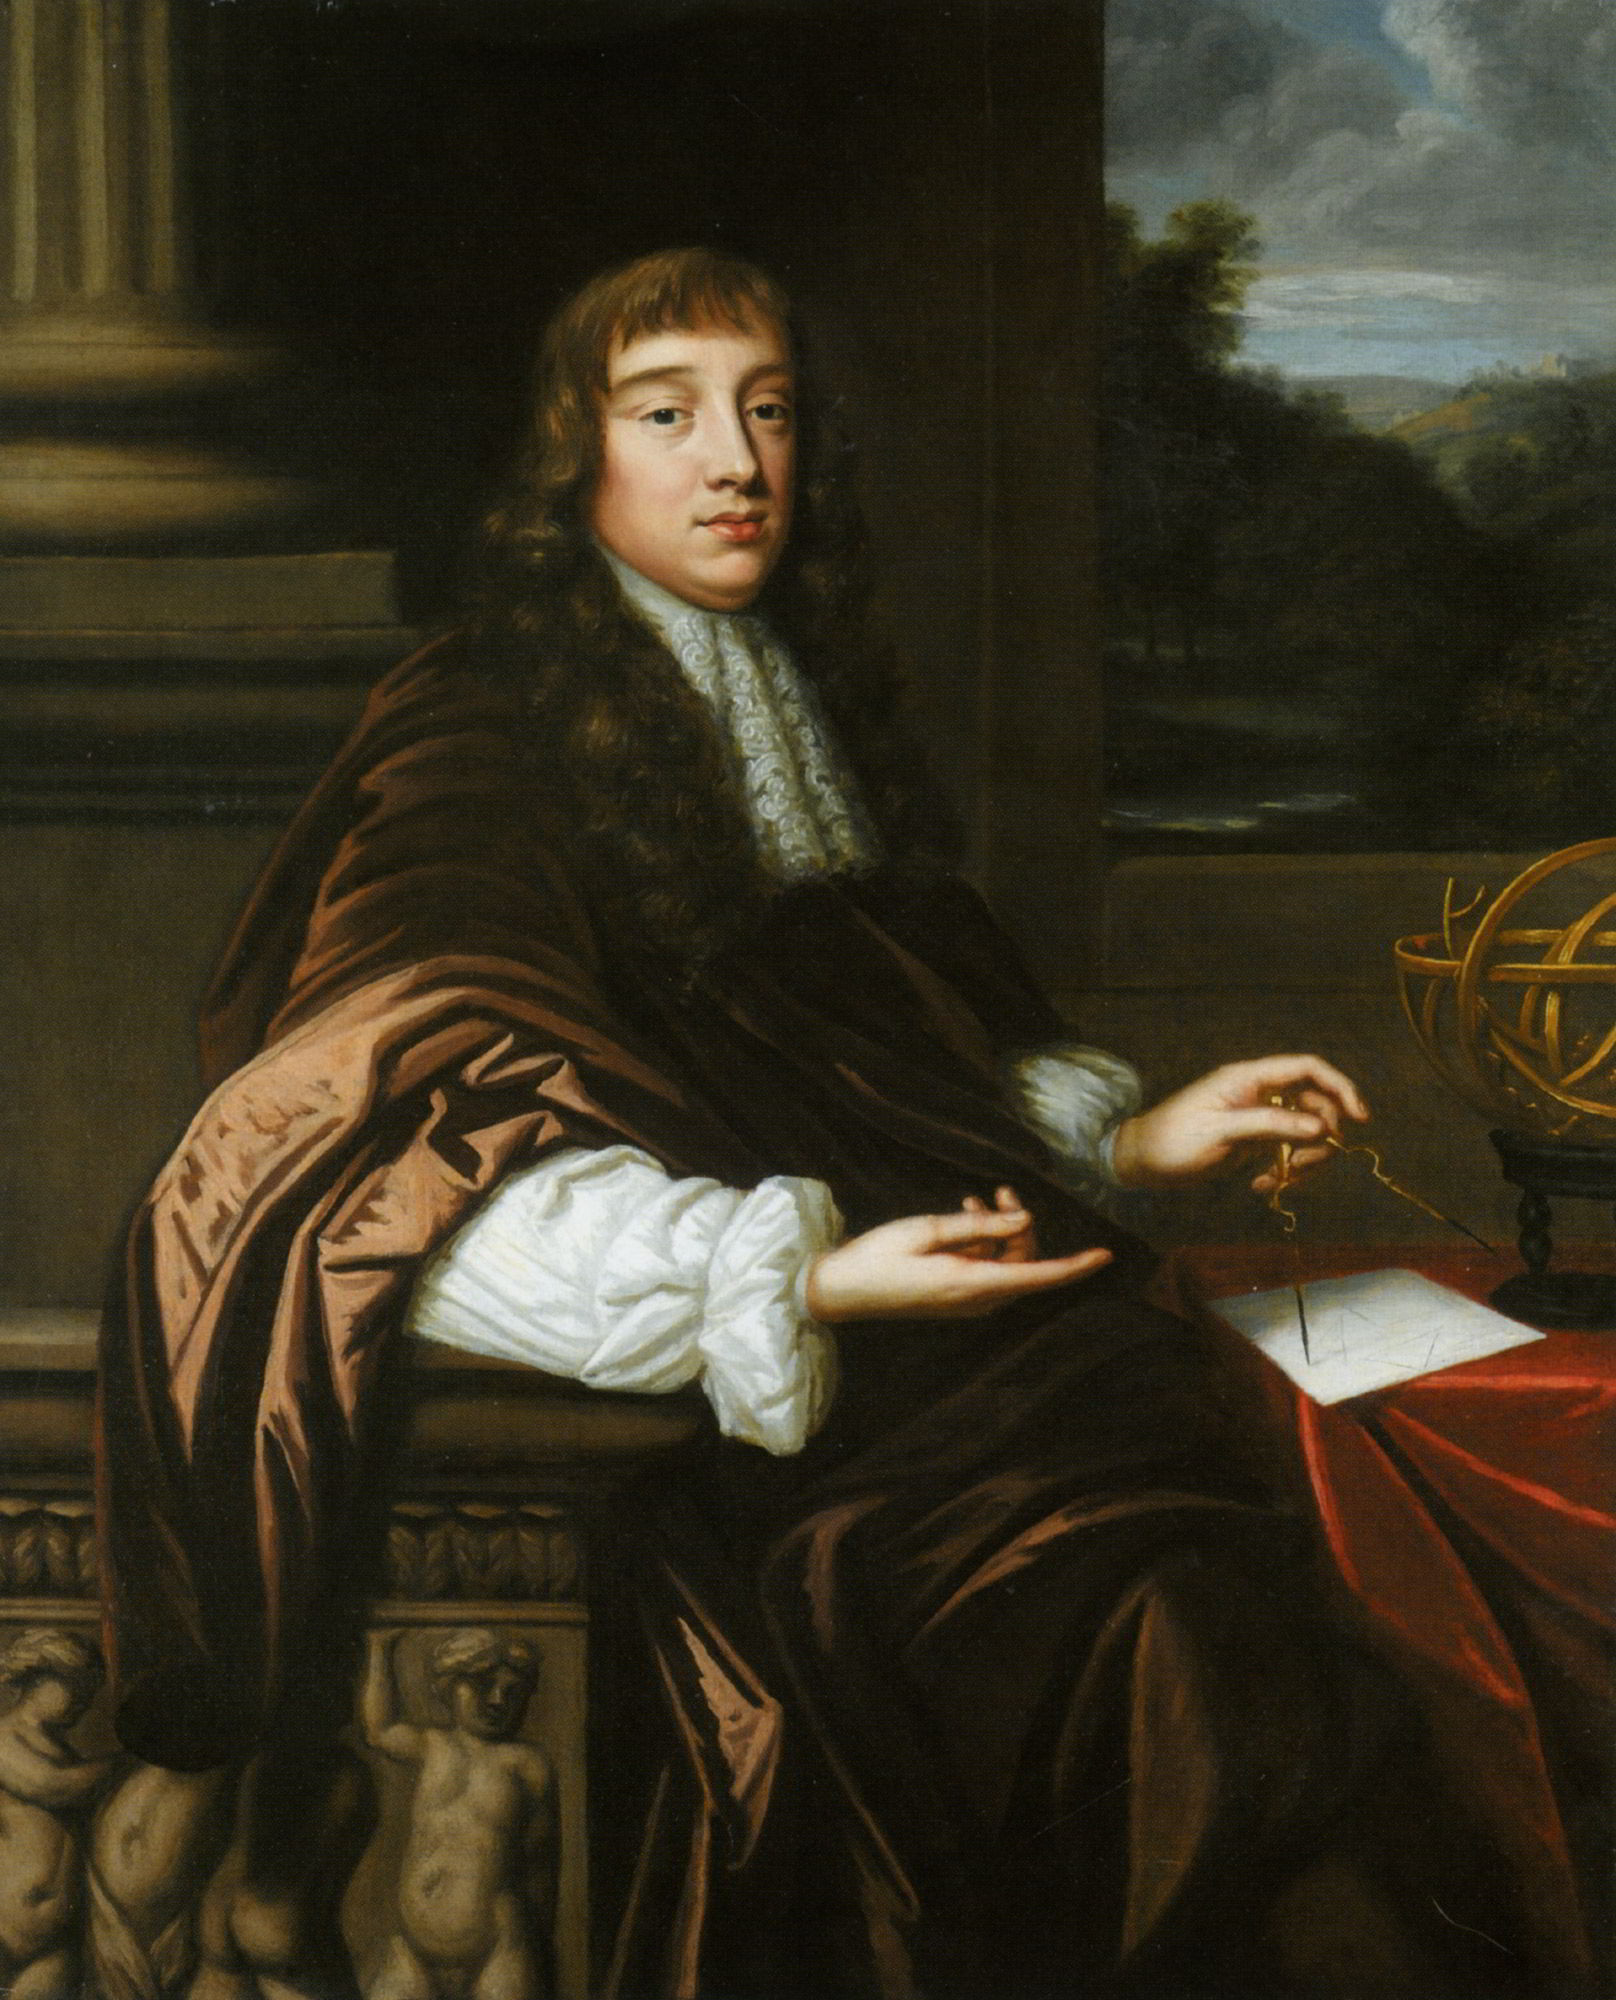
\includegraphics[width=0.4\textwidth]{../figures/robert hooke.jpg}
    \caption{Robert Hooke invented the simple microscope to look at thin pieces of cork tree. Classical cell theory was proposed by Schwann, Schleiden, and Virchow.}
\end{figure}

\section{Prokaryote and Eukaryote}
Organisms are divided into two types: prokaryote and eukaryote. 
\begin{definition}[Prokaryote]
    Organisms that have cells which contain \textbf{no nucleus}. 
\end{definition}

\begin{definition}[Eukaryote]
    Organisms that have cells which contain \textbf{a nucleus}. These fit under either \textbf{unicellular} or \textbf{multicellular}, meaning one nucleus and more than one nucleus, respectively.
\end{definition}

\begin{center}
\begin{forest}
    [Types of Organisms 
        [\textbf{Prokaryote}
            [Bacteria]
            [Archea]
        ]
        [\textbf{Eukaryote}
            [Unicellular
                [Protists
                    [Amoeba]
                    [Algae]
                    [Paramecium]
                ]
            ]
            [Multicellular
                [Animals]
                [Plants]
                [Fungi]
            ]
        ]
    ]
\end{forest}
\end{center}

\section{Organelles}
\begin{definition}[Organelles]
    An organelle is a small structure in a cell that is surrounded by a membrane and has a specific function.
\end{definition}

Basically, that organelles act like the organs in your body but instead it is for the cell. There are many different organelles, varying for plants and animals.

\subsection{Cell Membrane}
\begin{definition}[Cell Membrane]
    The cell membrane is like the outer wall of the cell. It is semi-permeable, meaning it allows only certain substances/materials through. See Figure \ref{fig:cell-membrane}. 
\end{definition}

The cell membrane is made of a double layer of lipids. A lipid is a fat-like molecule that does not dissolve in water. 

\begin{figure}[H]
\centering
    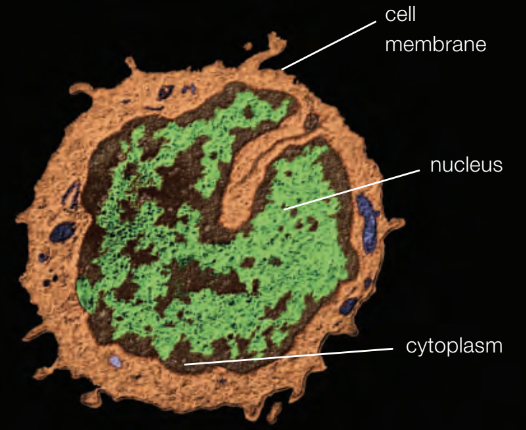
\includegraphics[width=0.5\textwidth]{../figures/cell membrane}
    \caption{A cell showing the cell membrane, cytoplasm, and large nucleus.}
    \label{fig:cell-membrane}
\end{figure}

\subsection{Cytoplasm}
\begin{definition}[Cytoplasm]
    The cytoplasm is a gel-like substance that fills the cell and surrounds organelles. Cytoplasm contains the nutrients required by the cell to carry on its life purposes. See Figure \ref{fig:cell-membrane}. 
\end{definition}

All organelles are suspended in cytoplasm. The physical nature of the cytoplasm allows the nutrients and organelles to move within the cell.

\subsection{Nucleus}
\begin{definition}[Nucleus]
    The nucleus is the control center of the cell. It controls all activities in the cell, including growth and reproduction. One important thing is that it contains nearly all of the cell's DNA. See Figure \ref{fig:nucleus}.
\end{definition}

\begin{note}{ }
    DNA stands for deoxyribonucleic acid. DNA is very important to the cell because it contains the coded information for making protesins and other molecules. Proteins servec many purposes and are found in various locations of the cell.
\end{note}

\begin{figure}[H]
\centering
    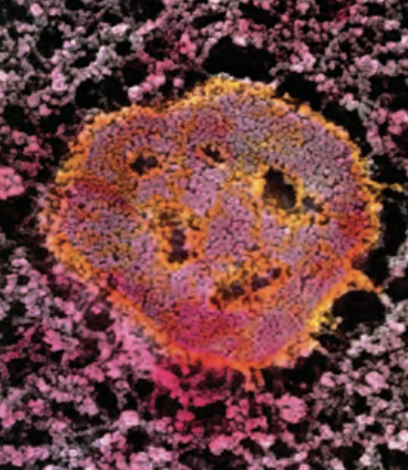
\includegraphics[width=0.3\textwidth]{../figures/nucleus.png}
    \caption{The nucleus and chromatin in a human cell, as seen through an electron microscope.}
    \label{fig:nucleus}
\end{figure}

\subsection{Vesicles}
\begin{definition}[Vesicles]
    Vesicles are membrane-bound organelles that store nutrients, waste, and other substances used by the cell. Vesicles can fuse with the cell membrane. 
\end{definition}

\subsection{Vacuoles}
\begin{definition}[Vacuoles]
    Vacuoles are basically vesicles but bigger and do not fuse with the cell membrae. You can think of them as the storage system. See Figure \ref{fig:vacuoles}./ 
\end{definition}

\begin{figure}[H]
\centering
    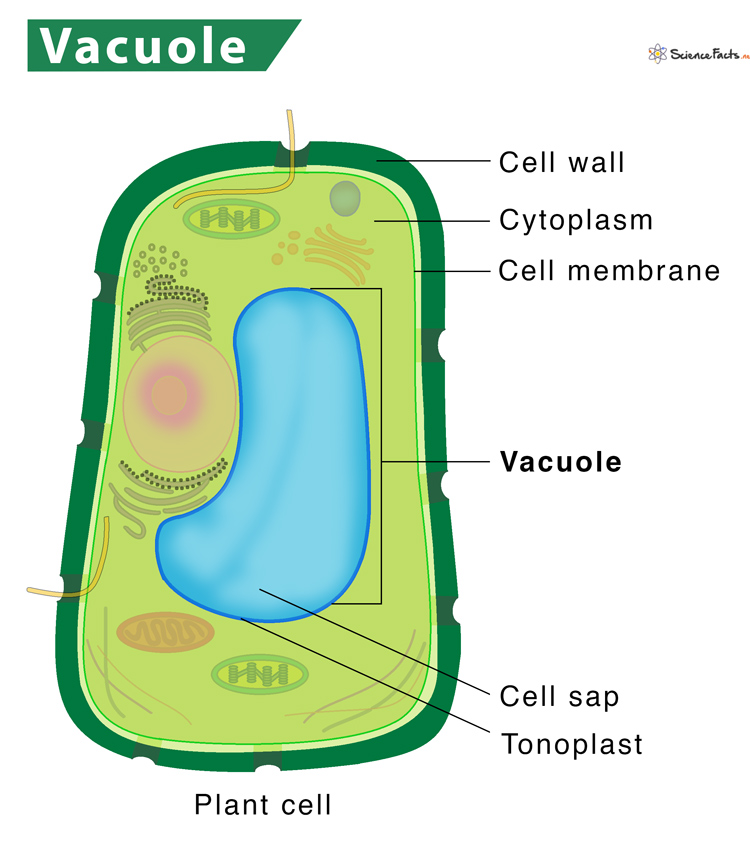
\includegraphics[width=0.4\textwidth]{../figures/vacuole.jpg}
    \caption{A vacuole inside of a plant. You can tell it is inside of a plant because a plant only has ONE large vacuole.}
    \label{fig:vacuoles}
\end{figure}

\subsection{Mitochondria}
\begin{definition}[Mitochondria]
    The powerhouse of the cell. The mitochondria supplies the cell with energy by converting the chemical energy within sugar into energy that the cell can use. See Figure \ref{fig:mitochondria}.
\end{definition}

\begin{figure}[H]
\centering
    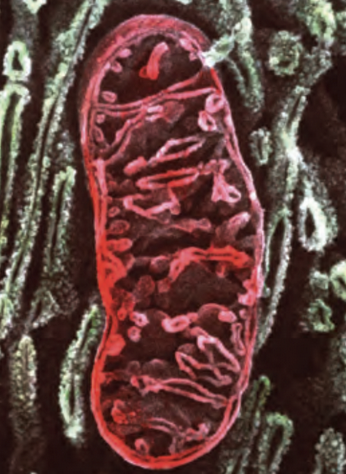
\includegraphics[width=0.3\textwidth]{../figures/mitochondria.png}
    \caption{A mitochondrion, as seen through an electron micoroscope.}
    \label{fig:mitochondria}
\end{figure}

\subsection{Lysosomes}
\begin{definition}[Lysosomes]
    Lysosomes are organelles where digestion takes place. They are small organelles that are filled with enzymes. Lysosomes also break down invading bacteria and damaged cell organelles. See Figure \ref{fig:lysosomes}. 
\end{definition}

Essentially, they work as the clean-up system in the cell.

\begin{figure}[H]
\centering
    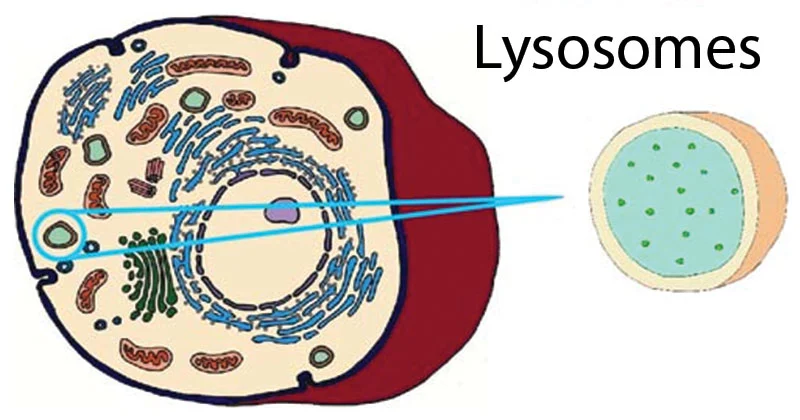
\includegraphics[width=0.5\textwidth]{../figures/lysosomes.png}
    \caption{Lysosomes}
    \label{fig:lysosomes}
\end{figure}

\begin{note}{Enzyme}
    An enzyme is a protein that can speed up chemical reactions in the cell.
\end{note}

\subsection{Rough Endoplasmic Reticulum}
\begin{definition}[Rough Endoplasmic Reticulum]
    The rough endoplasmic reticulum is like a conveyor belt for proteins and nutrients that are destined for the nucleus. The rough endoplasmic reticulum is studded with ribosomes which allows it to easily transport proteins once they are made. You can think of the rough endoplasmic reticulum as an organelle that synthesizes proteins. See Figure \ref{fig:endoplasmic-reticulum}. 
\end{definition}

\begin{figure}[H]
\centering
    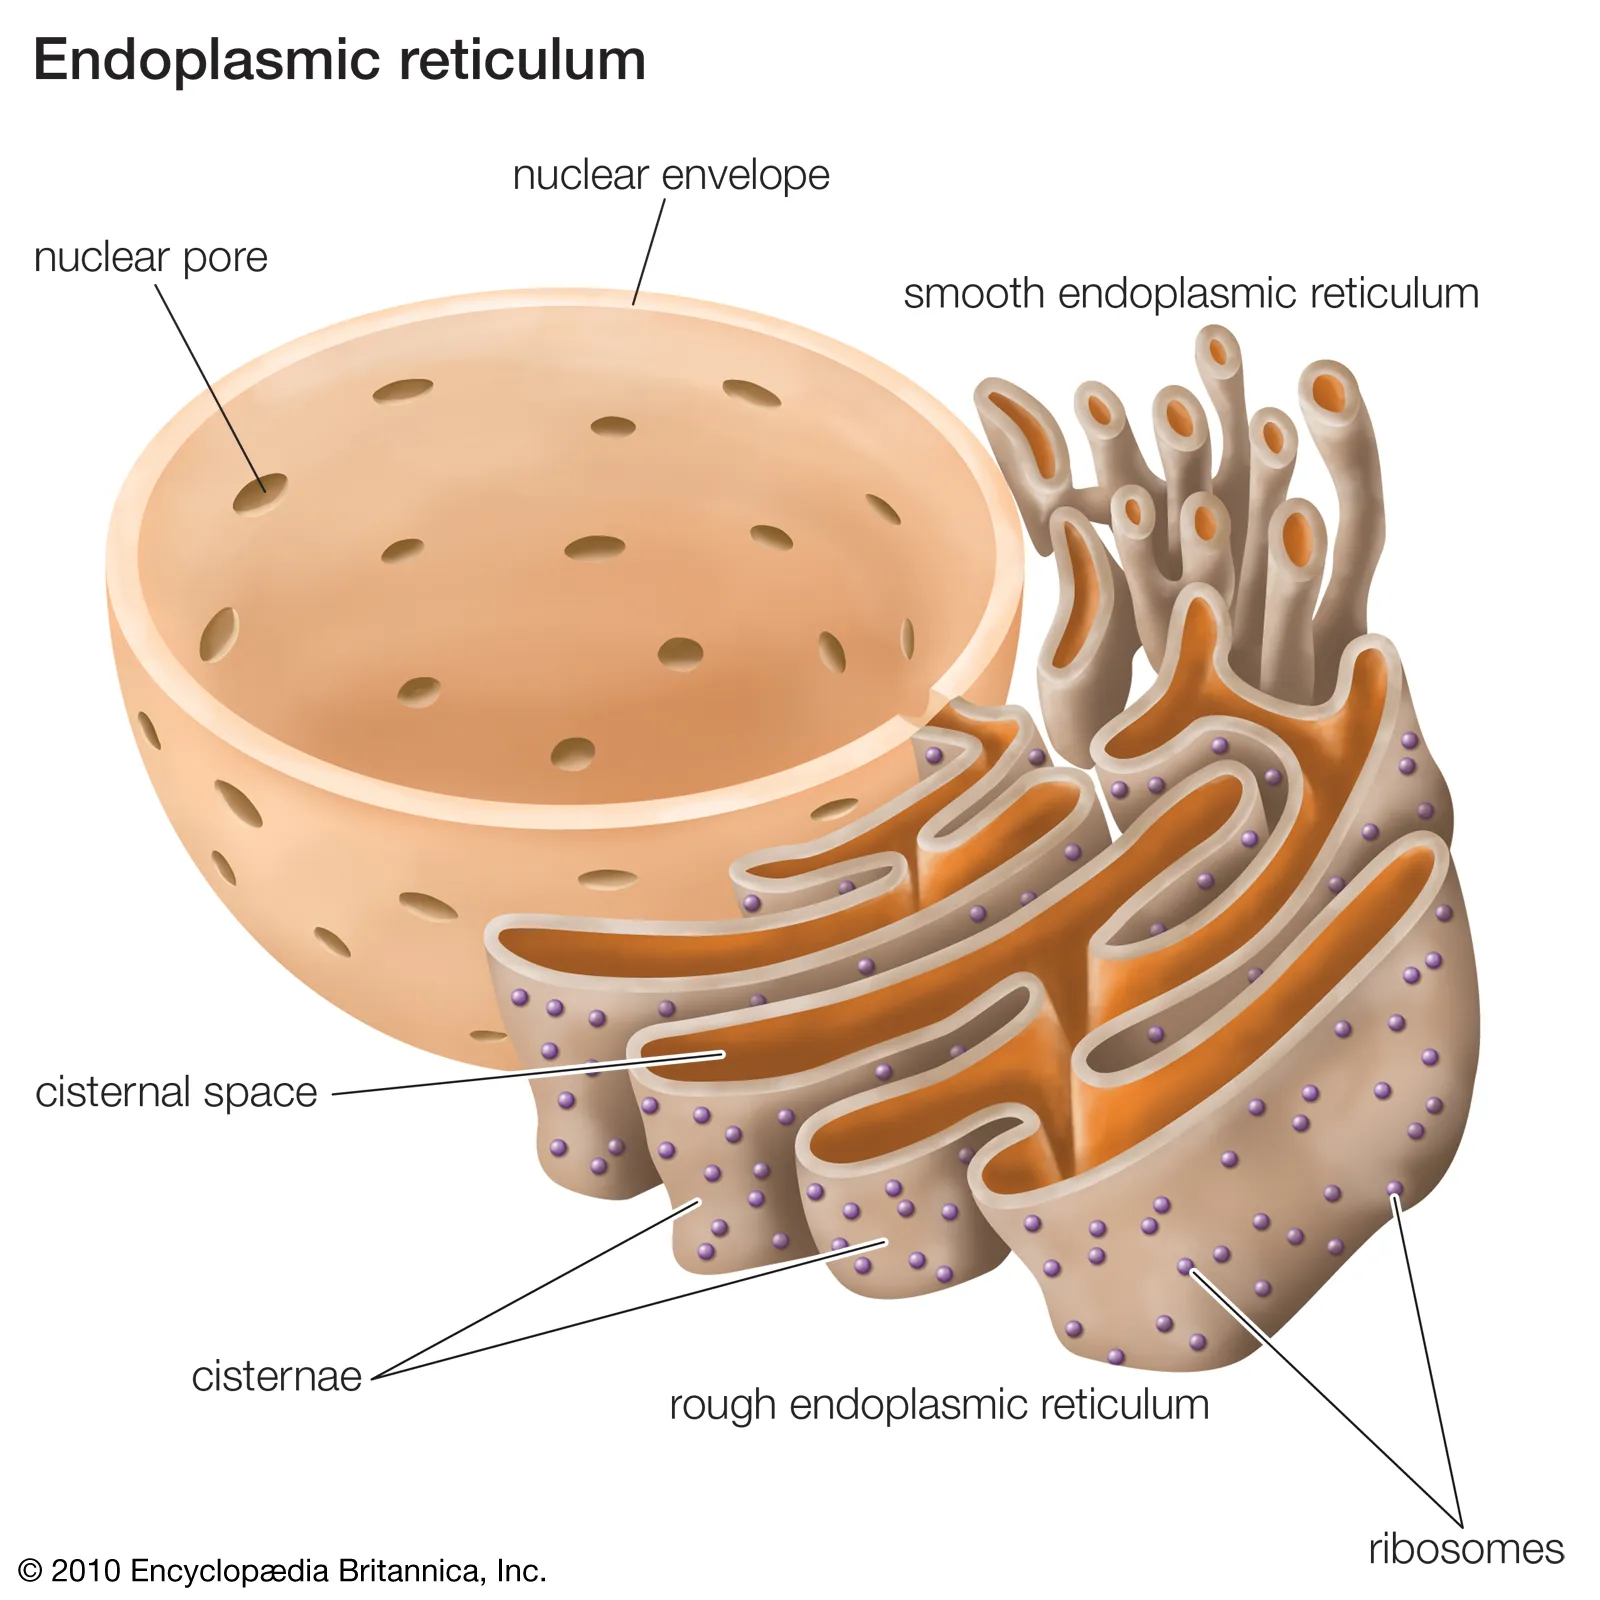
\includegraphics[width=0.5\textwidth]{../figures/endoplasmic-reticulum.png}
    \caption{The rough and smooth endoplasmic reticulums.}
    \label{fig:endoplasmic-reticulum}
\end{figure}

\subsection{Smooth Endoplasmic Reticulum}
\begin{definition}[Smooth Endoplasmic Reticulum]
    Similar to the smooth endoplasmic reticulum, except that it lacks ribosomes and is involved in lipid metabolism, including the synthesis of phospholipids, steroids, and other lipids. See Figure \ref{fig:endoplasmic-reticulum}. 
\end{definition}

\begin{note}{Lipid}
    Lipid is another word for "fat".
\end{note}

Basically, the rough endoplasmic reticulum is involved in protein synthesis and processing, whereas the smooth endoplasmic reticulum is involved in lipid metabolism and detoxification. The main difference is the prescence of ribosomes in both cases.

\subsection{Ribosomes}
\begin{definition}[Ribosomes]
    Ribosomes are small, dense-looking organelles that may be attached to the rough endoplasmic reticulum or free in the cytoplasm. Ribosomes are the sites where the proteins are assembled. 
\end{definition}

\subsection{Golgi Body/Apparatus}
\begin{definition}[Golgi Body/Apparatus]
    The golgi body receives proteins from the endoplasmic reticulum and processes them for removal from the cell. They modify, sort, and package these proteins for delivery throughout the cell or outside of the cell. The golgi body looks like a stack of flattened membranes (see Figure \ref{fig:golgi-body}).
\end{definition}

\begin{figure}[H]
\centering
    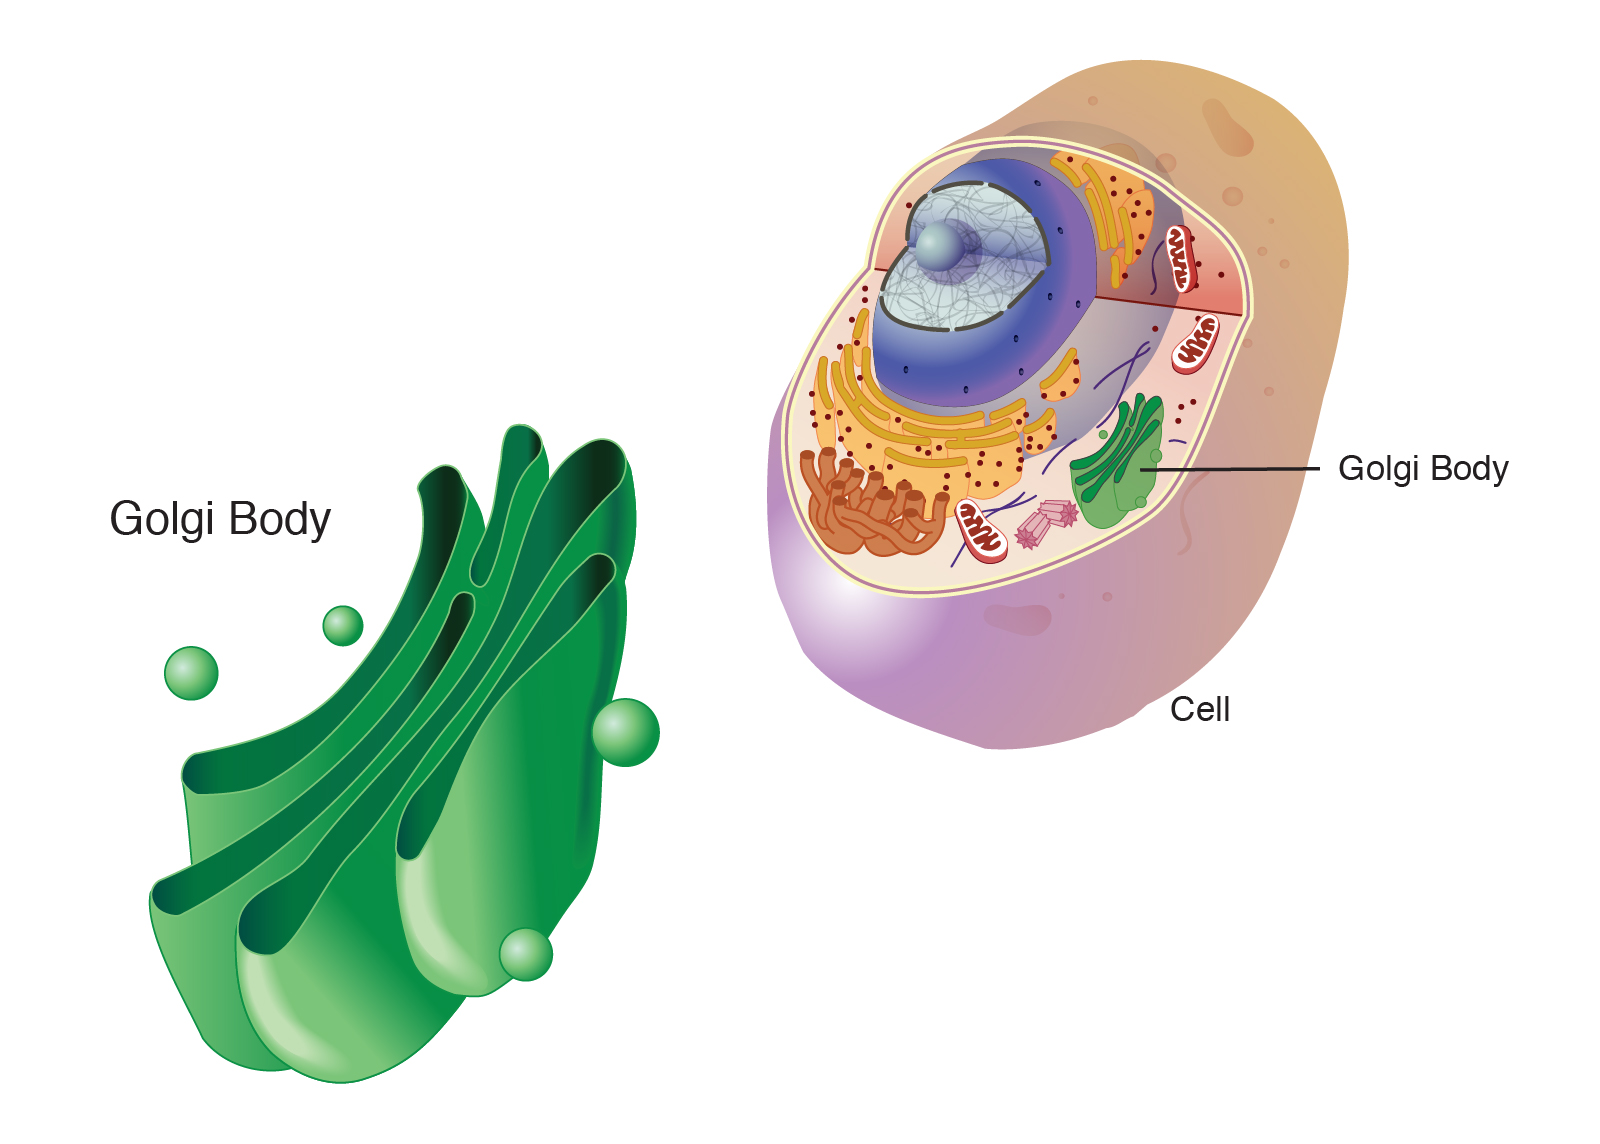
\includegraphics[width=0.5\textwidth]{../figures/golgi_body.jpg}
    \caption{Golgi body.}
    \label{fig:golgi-body}
\end{figure}

\subsection{Cytoskeleton}
\begin{definition}[Cytoskeleton]
    The cytoskeleton gives structure to the cell and is made of protein filaments.
\end{definition}

\subsection{Chloroplast}
\begin{definition}[Chloroplast]
    Chloroplasts are only found in plants cells and some algae. Contains a pigment called chlorophyll that absorbs light and energy to undergo photosynthesis 
    \[
        \ce{6CO2}+ \ce{6H2O}+ \text{light}\to \ce{C6H12O6}+ \ce{6O2}
    \]
\end{definition}

\begin{note}{Thylakoids}
Chloroplasts are made of little sacs called \textbf{thylakoids}. A stack of thylakoids is called a \textbf{granum}. You can think of the thylakoids as solar panels.
\end{note}

\section{Histology}
\begin{definition}[Histology]
    A branch of study that concerns the study of biological tissues using a microscope.
\end{definition}

Thin slices are placed on microscope slides to be visualized underneath a microscope. Specimens stained with various data types and chemicals to visualize organelles. 

\section{Asexual vs Sexual}
\subsection{Asexual}
\begin{definition}[Asexual]
    Producing from only one parent. Exact same genes/DNA of the parent cell.
\end{definition}

\textbf{Advantages:}
\begin{itemize}
    \item{Only need one parent.}
    \item{Very efficient; not many resources are required to initiate asexual reproduction.}
    \item{Happens very quicktly.}
\end{itemize}

\textbf{Disadvantages:}
\begin{itemize}
    \item{Decreases overall genetic resilience of the population.}
    \item{In turn there will be issues with diseases wiping out the entire population. This is because if there is say ebola, then it will whipe out everyone, since everyone is the same. If it kills one person, it will kill everyone too.}
\end{itemize}

\subsection{Sexual}
\begin{definition}[Sexual]
    Producing offspring by fusion of two gametes (egg and sperm). Offspring will have genetic material from both parents and newer cells will be created threw mitosis.
\end{definition}

\textbf{Advantages:}
\begin{itemize}
    \item{Genetic variability of the population will be high.}
    \item{As a result, the population will be more resilient in the face of pathogens.}
    \item{For example, some people weren't affected at all by the bubonic plague because they had a slight variance in their genetics that made them immune to the disease.}
\end{itemize}

\textbf{Disadvantages:}
\begin{itemize}
    \item{Two parents are required; slower than asexual reproduction.}
    \item{Time and energy are required to find a suitable mate for reproduction.}
    \item{Not every individual in the population gets to reproduce. Example: fat and obese people have a lower chance to reproduce than muscular people.}
    \item{Genetically heritable conditions can be passed down. Example: diabetes.}
\end{itemize}



\section{The Cell Cycle}
\begin{definition}[Cell Cycle]
In your body, cells are constantly dying and being replenished. During much of the cell cycle, the cell prepares for \textbf{cell division}. The three stages are: 
\begin{enumerate}
\setlength\itemsep{0.5em}
    \item{Interphase}
    \item{Mitosis}
    \item{Cytokinesis}
\end{enumerate}
See Figure \ref{fig:cell-cycle}.
\end{definition}

Cell division occurs for the purpose of reproduction. There are two types, namely \textbf{asexual} and \textbf{sexual}.

\begin{figure}[H]
\centering
    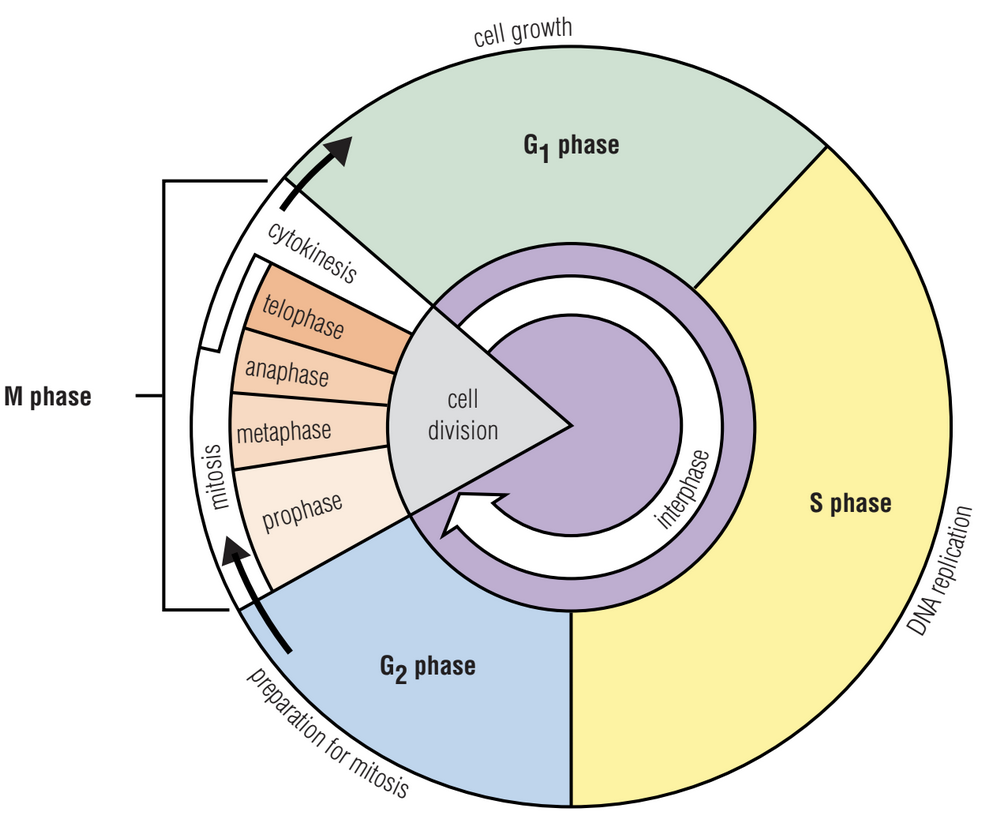
\includegraphics[width=0.8\textwidth]{../figures/cell cycle.png}
    \caption{The cell cycle has four phases. During most of the cell cycle, the cell is growing, replicating its DNA, and preparing for cell division.}
    \label{fig:cell-cycle}
\end{figure}

\subsection{Cell Division}
\begin{definition}[Cell Division]
    Cell division is the process by which a single cell divides into two or more daughter cells. This process is essential for the growth and maintenance of all living organisms.
\end{definition}

One method of cell division is known as \textbf{mitosis} (see Section \ref{sec:mitosis}).\\

Cell division allows organisms to \textbf{grow}. 
\begin{itemize}
    \item{Nutrients move through diffusion (high concentration to low concentration).}
    \item{Water enters and leaves the cell through osmosis (high concentration to low concentration).}
    \item{Cells need to divide to ensure a high surface area to maximize diffusion of nutrients/waste and osmosis of water.}
    \item{We need lots of cells that will cover a greater surface area because it speeds up the process of diffusion.}
\end{itemize}

Cell division allows organisms to \textbf{repair}.
\begin{itemize}
    \item{Organisms need to repair cells from damage or old age.}
    \begin{table}[h!] % delete [h!] if there are bugs
    
        %%% TABLE CONFIG %%% 
        \renewcommand{\arraystretch}{1.5} % changes vertical space for each cell 
        \setlength{\tabcolsep}{10pt} % changes horizontal space for each cell
        \setlength{\arrayrulewidth}{0.25mm}
    
        \begin{center}
            Repair Rate for Cells \\
            \vspace{0.5em}
            \begin{tabular}{|c|c|} % use r, l, c for right, left, center. use m{3cm} for middle width of 3cm, use  b{3cm} for bottom width of 3cm, and use p{3cm} for a top width of 3cm.  
            \hline
            Cell Type & Turnover Time \\ % two columns corresponding to two c's
            \hline
            Stomache &  2-4 days\\ % second row
            \hline
            Skin & 10-30 days\\ 
            \hline
            Red blood cells & 4 months \\ 
            \hline 
            Liver cells & 6-12 months\\ 
            \hline 
            Brain cells & Life time\\ 
            \hline
            \end{tabular}
        \end{center}
    \end{table}

    \item{Stages of skin regeneration:}
        \begin{itemize}
            \item{New skin cells.}
            \item{Coming to surface.}
            \item{Degeneration process.}
            \item{Dead skin cells.}
        \end{itemize}
\end{itemize}

\subsection{Chromosomes}
\begin{definition}[Chromosomes]
    Each chromosome is a long piece of DNA and protein. They carry genetic information in the form of genes. The number of chromosomes between each organism varies. Chromosomes are only visible when the cell is dividing. See Figure \ref{fig:chromosomes}.
\end{definition}
\begin{figure}[H]
\centering
    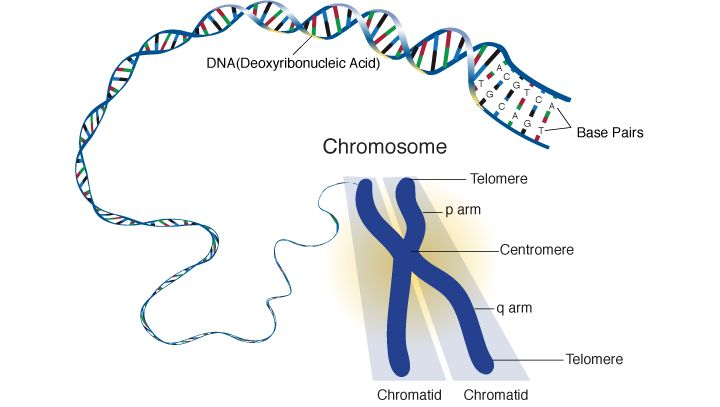
\includegraphics[width=\textwidth]{../figures/chromosomes.jpg}
    \caption{Chromosomes.}
    \label{fig:chromosomes}
\end{figure}

Before cell division can occur, each chromosome is copied, as shown in Figure \ref{fig:textbook-chromosomes}. The chromosome consists of two identical copies, can \textbf{sister chromatids}. When the cell divides, one chromatid goes to each of the new cells. 

\begin{figure}[H]
\centering
    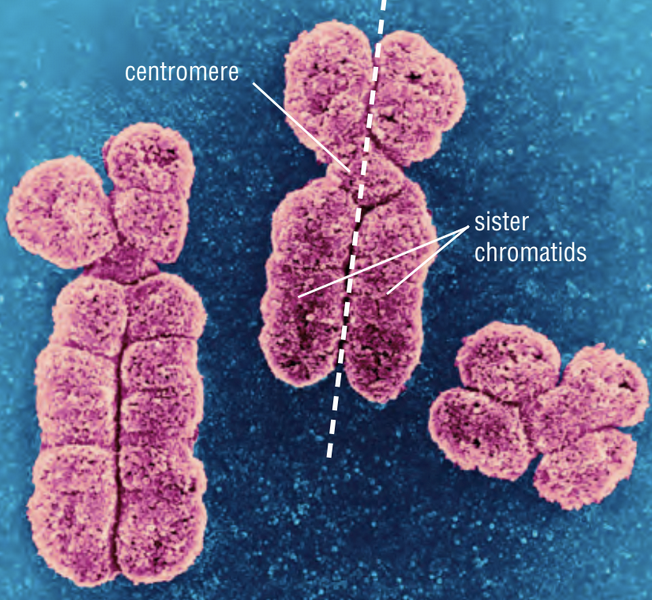
\includegraphics[width=0.5\textwidth]{../figures/textbook-chromosomes}
    \caption{Each chromosome consists of two identical sister chromatids. The \textbf{centromere} is where the sister chromatids attach.}
    \label{fig:textbook-chromosomes}
\end{figure}

\subsection{Interphase}
\begin{definition}[Interphase]
    The cell spends the most time in interphase. This phase refers to a period where the cell carries out its regular cell functions. This stage prepares the cell for \textbf{mitosis}. There are three phases (in the particular order): 
    \begin{enumerate}
    \setlength\itemsep{0.5em}
        \item{ \textbf{G1 Phase}: the cell grows in size and carries out normal metabolic processes.}
        \item{ \textbf{S Phase}: DNA replication, resulting in the formation of two identical copies of the cell's genetic material.}
        \item{ \textbf{G2 Phase}: organelles are duplicated. The cell undergoes further growth and prepares for division by synthesizing proteins necessary for mitosis.}
        See Figure \ref{fig:interphase}.
    \end{enumerate}
\end{definition}

\begin{figure}[H]
    \centering
    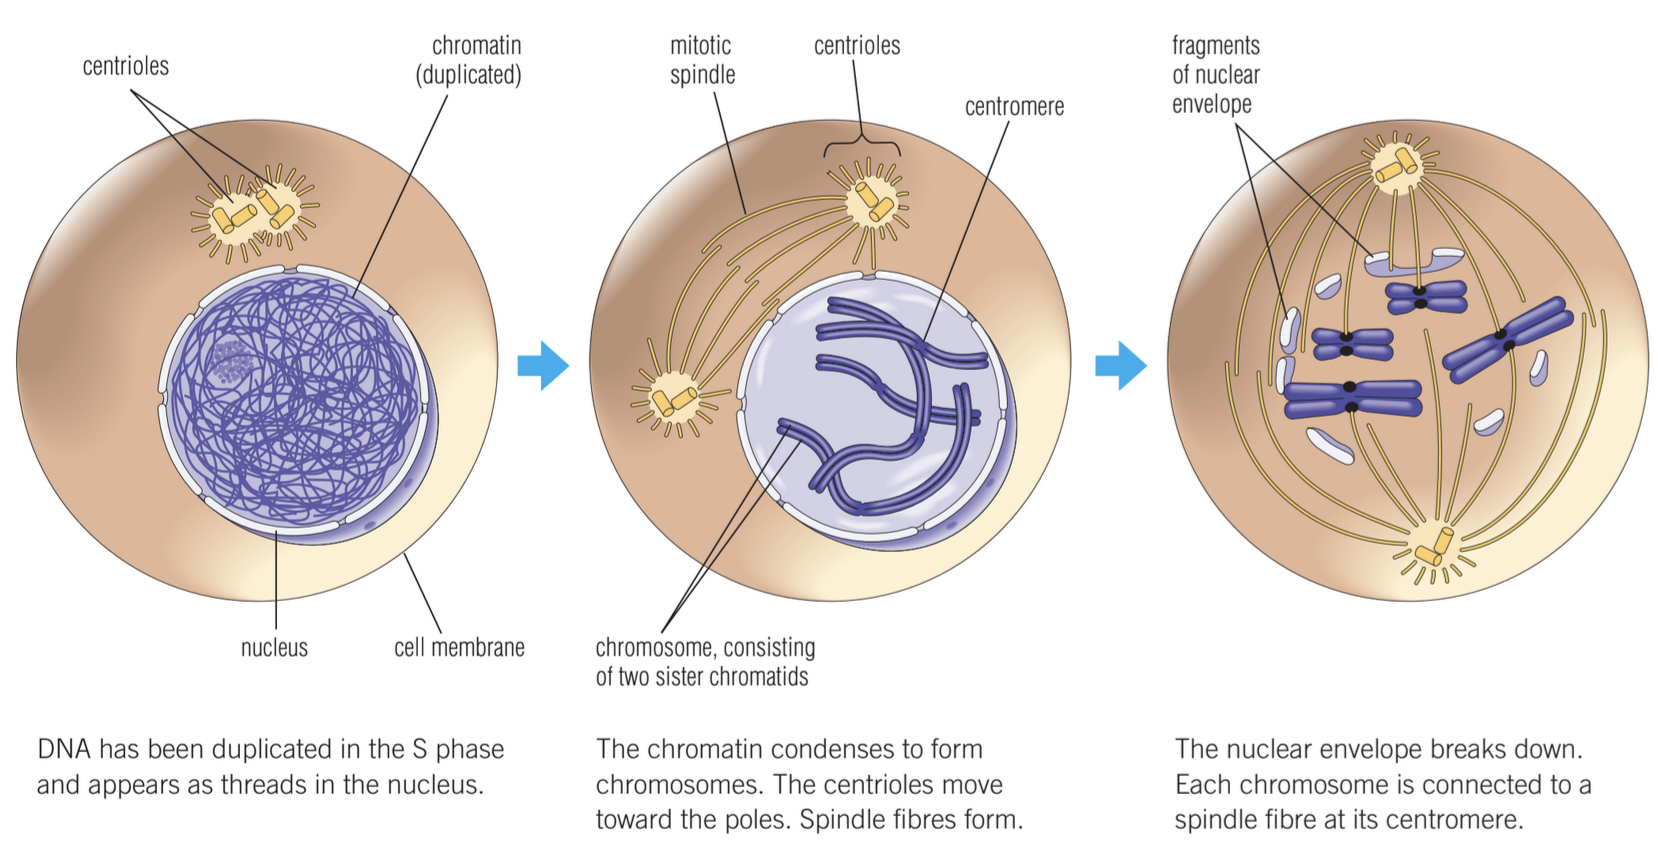
\includegraphics[width=\textwidth]{../figures/interphase.png}
    \caption{S phase and G2 phase.}
    \label{fig:interphase}
\end{figure}

\begin{note}{ }
    The cell grows until it reaches a certain size, at which it is healthier for the cell to undergo cell division.
\end{note}

\subsection{Mitosis}\label{sec:mitosis}
\begin{definition}[Mitosis]
    Mitosis is the stage in which DNA in the nucleus is divided. There are 4 stages of mitosis:
    \begin{enumerate}
    \setlength\itemsep{0.5em}
        \item{ \textbf{Prophase}: the chromosomes shorten and thicken.}
        \item{ \textbf{Metaphase}: chromosomes line up in the middle of the cell.}
        \item{ \textbf{Anaphase}: chromatids break apart at the centromere and move to opposite poles.}
        \item{ \textbf{Telophase}: two nuclei formed after nuclear envelopes reform around each group of chromosomes.}
    \end{enumerate}
    See Figure \ref{fig:mitosis}.
\end{definition}

\subsection{Cytokinesis}
\begin{definition}[Cytokinesis]
    Cytokinesis is the final stage of the cell cycle, where the cytoplasm is split and two daughter cells are formed. In an animal cell, this is done through the pinching of the membrane (cleavage furrow). In a plant cell, this is done through the formation of a cell plate.
\end{definition}

\begin{figure}[H]
\centering
    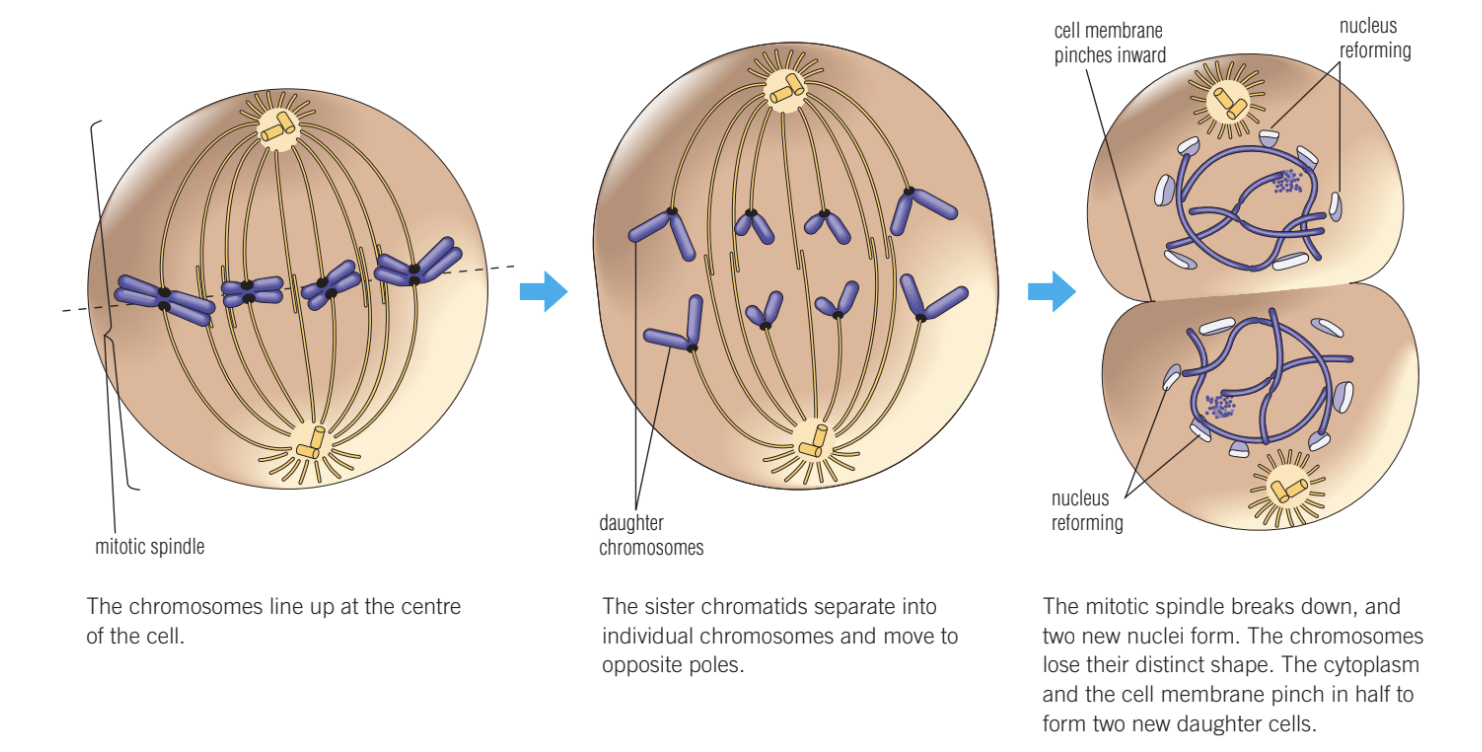
\includegraphics[width=\textwidth]{../figures/mitosis.png}
    \caption{Prophase then metaphase, anaphase, and telophase then cytokinesis.}
    \label{fig:mitosis}
\end{figure}

% \begin{problems}
%     \item{What is the purpose of the cell cycle?}
%         \begin{solution}
%             The cell cycle's purpose is to create new cells through cell division. Cell division allows organism to \textbf{grow} and \textbf{repair}.
%         \end{solution}
%     \item{Define the term ``interphase'' and describes its purpose.}
%         \begin{solution}
%             Interphase is the first phase in the cell cycle, and it is when the cell carries out its regular cell functions. The purpose of interphase is to get the cell ready to divide.
%         \end{solution}

%     \item{
%             \begin{2qu}
%                 \item{What is mitosis?}
%                     \begin{solution}
%                         Mitosis is a stage that contains 4 phases: prophase, metaphase, anaphase, and telophase. During this stage is where the cell actually divides, which is during telophase. After mitosis, a daughter cell of the parent cell is created. 
%                     \end{solution}
%                 \item{Why is mitosis important to the cell?}
%                     \begin{solution}
%                         Mitosis is important for \textbf{cell reproduction} (making new cells) and \textbf{growth} (optimization of surface are to cell volume ratio).
%                     \end{solution}
%             \end{2qu}
%         }

%     \item{Define and distinguish between the following terms: chromosome, centromere, and sister chromatids.}
%         \begin{solution}
%             \textbf{Chromosome}:
%             \begin{itemize}
%                 \item{Carries genetic information in the form of DNA.}
%                 \item{Made up of a long, coiled strand of DNA that is tighly packed around proteins.}
%                 \item{Comprised of two sister chromatids.}
%                 \item{Made up of chromatin.}
%             \end{itemize}
%             \textbf{Centromere}:
%             \begin{itemize}
%                 \item{The part that attaches the sister chromatids during prophase and metaphase.}
%             \end{itemize}
%             \textbf{Sister Chromatids:}
%             \begin{itemize}
%                 \item{Two identical copies of a single chromosome thar are produced during DNA replication.}
%                 \item{The sister chromatids are separated during anaphase.}
%                 \item{Attached at the center with a centromere during prophase and metaphase.}
%             \end{itemize}
%         \end{solution}

%     \item{Explain the meaning and importance of the term ``cytokinesis''.}
%         \begin{solution}
%             Cytokinesis is the final stage of the cell cycle, where the cytoplasm is split and two daughter cells are formed. In an animal cell, this is done through the pinching of the membrane (cleavage furrow). In a plant cell, this is done through the formation of a cell plate.
%         \end{solution}
% \end{problems}

\end{document}
